%==============================================================================
\section{Effects of Advanced Optical Modules}
\label{sec:om_effects}
%==============================================================================

In Sec.~\ref{sec:Gen2DOM}, two different concepts to substantially improve the 
optical modules have been introduced, prototypes of both are supposed to be 
deployed in PINGU: the mDOM that has several small PMTs instead of a single 
large one, and the WOM, where the effective area of a single small PMT is 
enhanced drastically by passive components. In this chapter, PINGU will be
modelled as it was built completely from these next-generation optical modules. 
Then the possible benefits for the experiment's outcome can be analysed.

\subsection{mDOM: Eliminating the Noise}
\label{sec:mdom_effect}

\begin{figure}[thp]
 \centering
  \subfloat[\label{fig:sigma_vs_time_mDOM}]
   {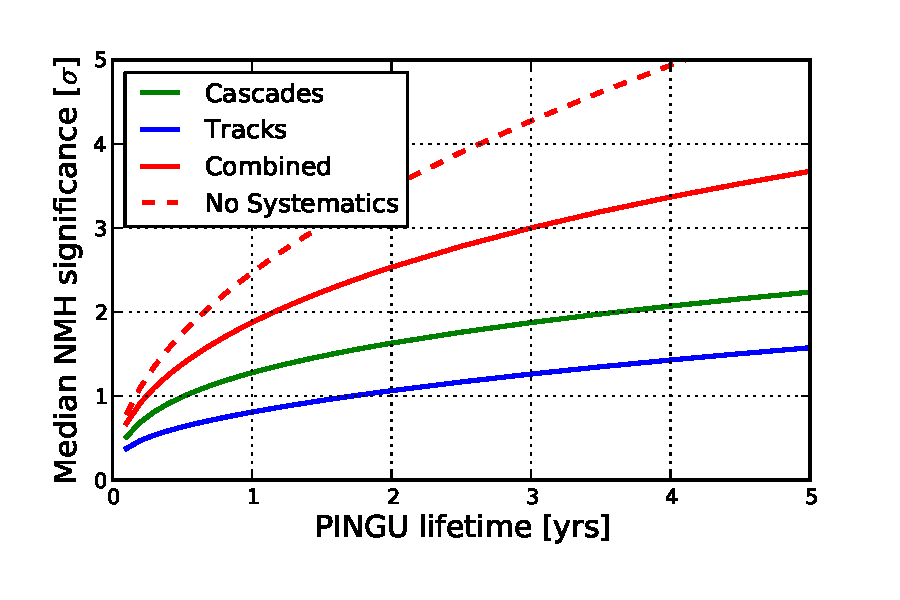
\includegraphics[width=0.495\linewidth]{sigma_vs_time_mDOM}}
  \subfloat[\label{fig:covmat_mDOM}]
   {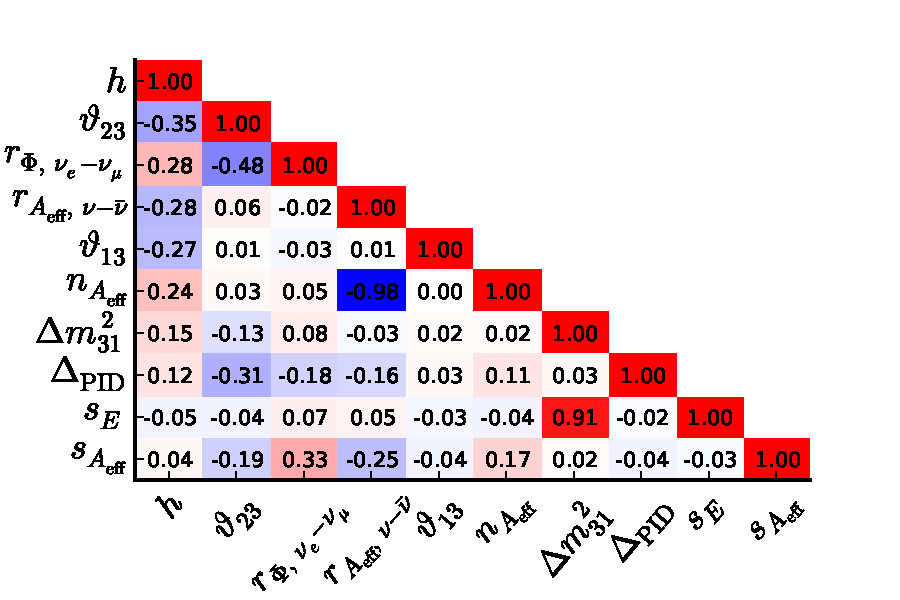
\includegraphics[width=0.495\linewidth]{CovMat_PINGU_mDOM}}
 \caption{\protect\subref{fig:sigma_vs_time_mDOM} Evolution of PINGU's expected
          mass hierarchy significance with time and
          \protect\subref{fig:covmat_mDOM} full correlation matrix for
          PINGU assuming reconstruction and particle identification as in
          geometry V15, \ie no module noise.}
 \label{fig:time_covmat_mDOM}
\end{figure}

\begin{figure}[hbp]
 \centering
 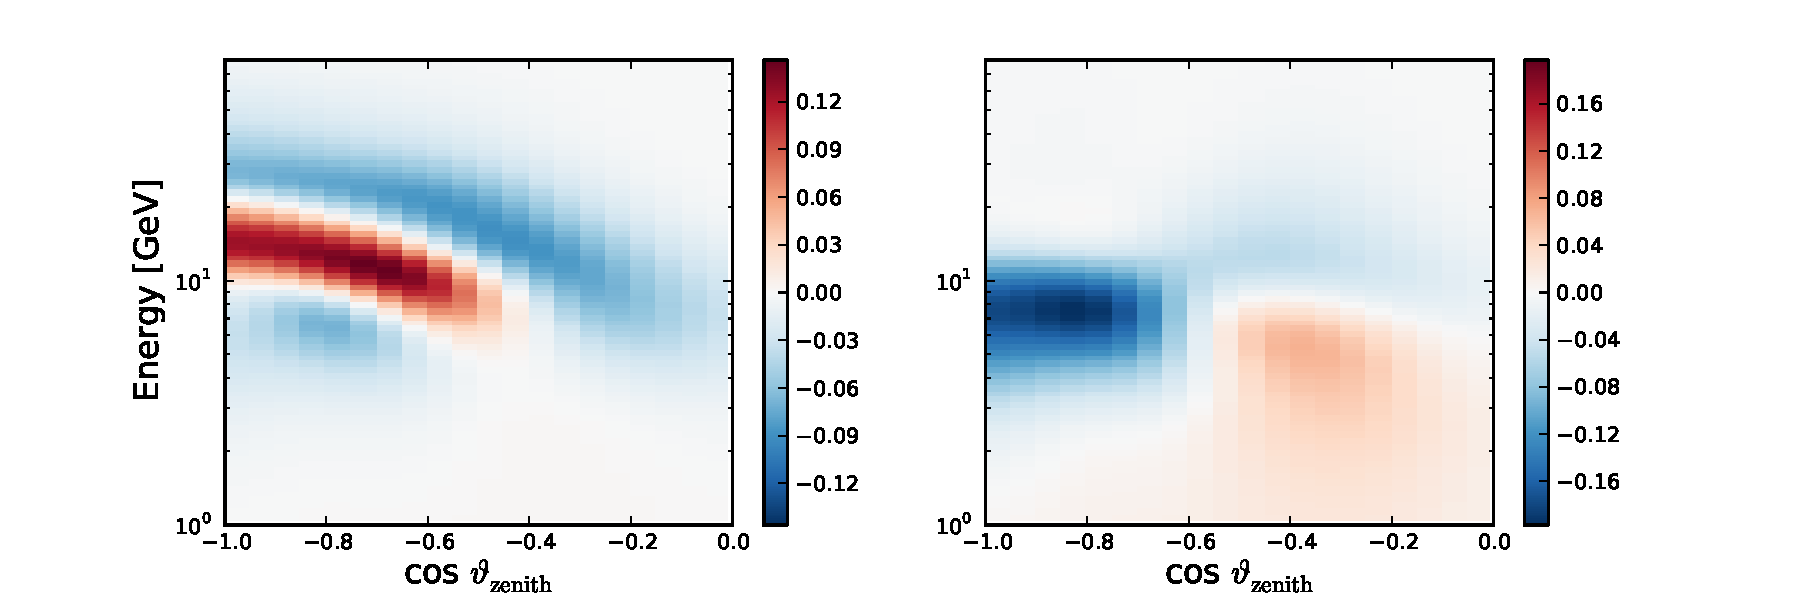
\includegraphics[width=\linewidth]{akhmedov_mDOM}
 \caption{\delchi distribution in the track (left) and cascade (right) channels
          assuming reconstruction and particle identification as in geometry
          V15, \ie no module noise.}
 \label{fig:akhmedov_mDOM}
\end{figure}

\noindent
The segmented photosensitive area of the mDOM will allow for an almost perfect
rejection of noise hits. Thus the event signatures will be clearer, leading to
an improved reconstruction and particle identification. In \papa, this can be
modelled by using the parametrised reconstruction functions and event
classification extracted from the Monte Carlo data for geometry V15, which was
erroneously produced without simulating noise. As the difference to geometry
V36 in terms of module density---which is crucial for the reconstruction
performance---is rather small\footnote{Geometry V36 has a horizontal string
spacing of 22\,m and a vertical module spacing of 3\,m, while in V15 string and
module spacing are 20\,m and 5\,m, respectively.}, the resulting
parametrisations, written out in App.~\ref{app:reco_V15} and
\ref{app:PID_threechannel}, respectively, should give a good approximation of
what to expect for the baseline geometry V36 with fully suppressed noise.

The resulting significance as function of lifetime and the correlation matrix
are shown in Fig.~\ref{fig:time_covmat_mDOM}. Comparing this to the results for
the baseline settings in Fig.~\ref{fig:time_covmat}, only a very small
improvement can be observed. When looking at the correlation matrix, the most
obvious change is the increased impact of the mixing angle \thet{23} and the
flux ratio $r_{\Phi,\,\nue-\numu}$ on the mass hierarchy.

The reason for this
is that especially the cascade channel profits from the improved particle
identification, increasing its significance without systematics from
3.0\,$\sigma$ to 3.3\,$\sigma$\footnote{The full error listings are shown in
App.~\ref{app:fisher_mDOM}}, which is reflected by the increased significance
scale of the \delchi distribution in the cascade channel, shown in
Fig.~\ref{fig:akhmedov_mDOM}. As such a feature basically means more \nue-like
events being detected, it can of course be mimicked by a wrong relative
normalisation of the primary \nue and \numu fluxes or a stronger oscillation
from \numu to \nue, determined by the value of \thet{23}. Unfortunately, these
two parameters are insufficiently constrained by themselves, thus they can
partly ``absorb'' the gain in sensitivity to the mass hierarchy.


\subsection{WOM: Increasing the Photon Statistics}
\label{sec:wom_effect}

With its enhanced photosensitive area, the WOM will primarily increase the
number of photons detected per event. Since this is the driving parameter for
event reconstruction quality---the more photons are detected, the more
information is available for the reconstruction algorithm---more precise
reconstructions are expected especially at low energies, where photon
statistics are scarce.

To simulate the improvement resulting from a photon count increased by a factor
\phfac in \papa, the \emph{absolute} widths of the energy reconstruction
functions that are usually given by linear functions of the form
\begin{equation}
 \sigma_E( E) = a  E + b \quad,
\end{equation}
where $a$ and $b$ are constants determined by a fit (see
App.~\ref{app:reco_params}), are replaced by
\begin{equation}
 \sigma'_E( E) = a  E + b/\phfac \quad.
\end{equation}
The rationale behind this is that the \emph{relative} energy resolution is
assumed to be a function of the number of detected photons, which in turn is
directly proportional to the neutrino energy\footnote{The number of Cherenkov
photons is proportional to the total deposited energy, see
Sec.~\ref{sec:Cherenkov}.}. Thus increasing the number of detected photons by
\phfac means that an an event with the energy $E$ will now have the relative
energy resolution of an event of energy $\phfac\cdot E$:
\begin{eqnarray}
 \frac{\sigma'_E( E)}{ E} &=& \frac{\sigma_E(\phfac E)}{\phfac E}
  = \frac{a \phfac E + b \quad}{\phfac E} \\
  \Rightarrow \sigma'_E( E) &=& a  E + b/\phfac
\end{eqnarray}
For the \coszen resolution, the modification is more straightforward as one can
simply read out the parametrisations for the absolute widths at an energy
increased by the factor \phfac:
\begin{equation}
 \sigma'_{\cos\theta}(E) = \sigma_{\cos\theta}(\phfac\cdot E) \quad.
\end{equation}

In addition, the threshold for passing PINGU's event selection is expected to
become lower with an increasing number of photons per neutrino energy,
enhancing the event statistics at low energy. This effect is mimicked by scaling
the effective area at a given energy $E$ by the ratio of the selection
efficiencies $\varepsilon_\mathrm{sel}$ (as shown in
Fig.~\ref{fig:selection_eff}) at $E$ and $\phfac \cdot E$:
\begin{equation}
 \aeff'(E) = \aeff(E) \cdot \frac{\varepsilon_\mathrm{sel}(\phfac\cdot E)}
                                 {\varepsilon_\mathrm{sel}(E)}
\end{equation}
The scaling is applied for all flavours except from \nutau and \nutaubar CC
events as there the main feature is the kinematic cutoff due to the large mass
of the tau lepton (cf.\ Sec.~\ref{sec:cuts_step2}), which of course is
independent from the performance of the optical modules used in the detector.

This gives a conservative estimate as only effects after the actual triggering
of the detector are taken into account. Since the trigger condition essentially
is a certain number of photon hits being registered within a short time window,
the trigger threshold itself does sink as well, enhancing the overall effect.
Yet as the available amount of MC events before triggering is insufficient to
quantify this, the lower trigger threshold will be neglected.

Finally, a similar reasoning can be applied for the particle identification
efficiency, thus the PID functions will be read off at the scaled energy as
well:
\begin{equation}
 P'_\mathrm{PID}(E) = P'_\mathrm{PID}(\phfac\cdot E)
\end{equation}

\begin{figure}[thp]
 \centering
 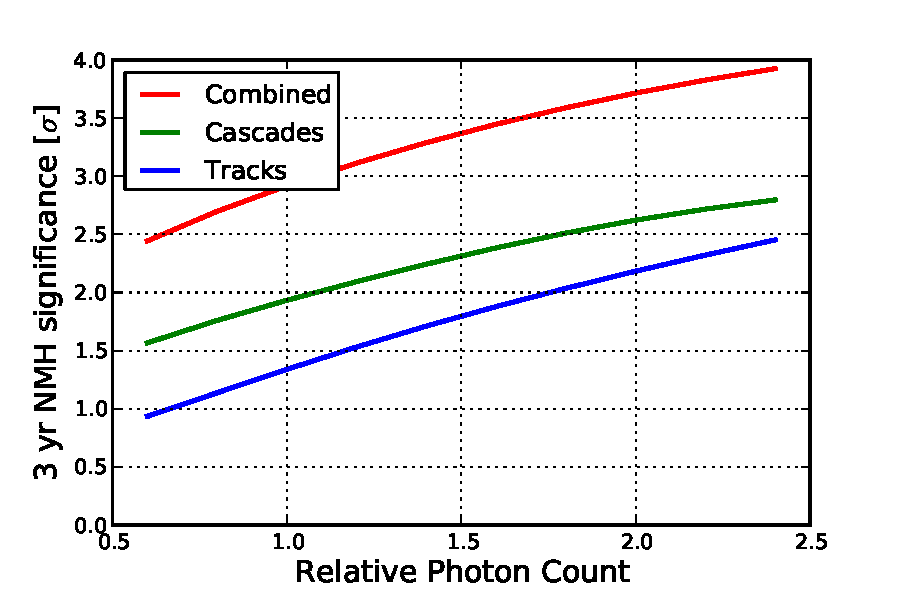
\includegraphics[width=0.7\linewidth]{increase_photon_count}
 \caption{Relative expected three-year significance for the mass hierarchy 
          as a function of \phfac.}
 \label{fig:increase_photon_count}
\end{figure}

The median three-year significance for the mass hierarchy is shown as a
function of \phfac in Fig.~\ref{fig:increase_photon_count}. As expected, the
mass hierarchy significance increases with the photon statistics as a result of
the improved resolutions. When the photon statistics are doubled, \ie $\phfac =
2$, it reaches 3.7\,$\sigma$, an increase of almost 30\,\%. Looking at the
track and cascade channels separately, the tracks are profiting slightly more
from the higher number of photons. This emphasises the fact that the track
channel is more affected by systematics (cf.\ Sec.~\ref{sec:results_baseline}),
which can be resolved better if the events are reconstructed more precisely.